%======================================================================
\NEWSEC
%======================================================================

\subsection{\ssCompare}

\usebackgroundtemplate
{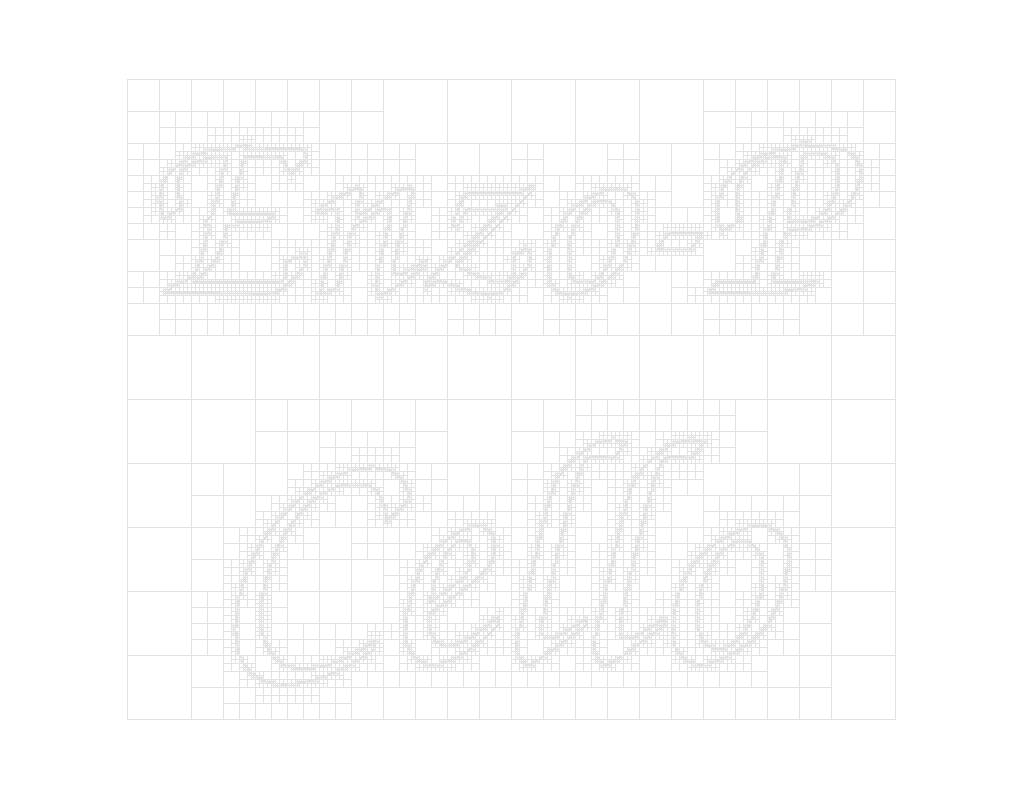
\includegraphics[width=5in]{cello-background.png}}
\begin{frame}[fragile,label=ss-compare] 
% ----------------------------------------------------------------------
\secframetitle{\ssCompare}
%\framesubtitle{}
% ----------------------------------------------------------------------
\begin{center}
\rowcolors[]{1}{blue!5}{blue!10}
\begin{tabular}{l|cc} 
 & \textbf{\enzo} & \textbf{\enzopcello} \\ \hline
\uncover<2->{Parallelization} & \uncover<2->{MPI} & \uncover<2->{\charm} \\
\uncover<3->{AMR type}       & \uncover<3->{patch-based} & \uncover<3->{octree-based}   \\
\uncover<4->{AMR structure} & \uncover<4->{replicated} &\uncover<4->{ fully distributed}   \\
\uncover<5->{Time stepping} & \uncover<5->{level-adaptive} & \uncover<5->{block-adaptive$^*$}   \\
\uncover<6->{Block sizes} & \uncover<6->{varies widely} & \uncover<6->{constant}  \\
\uncover<7->{Task scheduling} & \uncover<7->{level-parallel} & \uncover<7->{dependency-driven}  \\
\uncover<8->{Load balancing} & \uncover<8->{patch migration} & \uncover<8->{\charm-based}  \\
%\uncover<9->{Data locality} & \uncover<9->{LB conflict} & \uncover<9->{no LB conflict}  \\ 
%\uncover<10->{Mesh quality} & \uncover<10->{level jumps} & \uncover<10->{2-to-1 constraint}  \\  \hline
\end{tabular} \\
\uncover<5->{\footnotesize $^*$ not implemented yet}
%  
% \ \\ \ \\
% \url{http://cello-project.org} \\
% NSF PHY-1104819, AST-0808184 \\
% $\qed$
\end{center}
\end{frame}

\usebackgroundtemplate
{}
